\chapter{Algoritmi}
\label{Geom_Algos}
%
\section{Struttura ad albero di tipo "\textit{Bounding Volume Hierarchy}"}
%
Una \ac{BVH} è una struttura ad albero su un insieme di oggetti geometrici. Tutti gli oggetti geometrici sono raccolti in volumi limite che formano i nodi fogliari dell'albero. Questi nodi vengono quindi raggruppati come piccoli insiemi e racchiusi in volumi di delimitazione più grandi. Questi, a loro volta, sono ancora raggruppati e racchiusi in altri volumi di delimitazione più grandi in modo ricorsivo, risultando infine in una struttura ad albero con un singolo volume di delimitazione nella parte superiore dell'albero. Le strutture \ac{BVH} vengono utilizzate per supportare in modo efficiente diverse operazioni su insiemi di oggetti geometrici, come ad esempio il rilevamento delle collisioni.

Il confinamento degli oggetti nei volumi di delimitazione e l'esecuzione di test di collisione su di essi, prima di effettuare il test della geometria dell'oggetto stesso, comporta una semplificazione del problema e un miglioramenti significativi delle prestazioni. Organizzando i volumi di delimitazione in una strutture \ac{BVH}, la complessità temporale (il numero di test eseguiti) può essere ridotta logaritmicamente nel numero di oggetti. Con una tale struttura, durante i test di collisione, i volumi secondari non devono essere esaminati se i loro volumi principali non sono intersecati.
%
\subsection{Struttura di tipo "\textit{Minimum Bounding Box}"}
In geometria, il rettangolo minimo o più piccolo (o \ac{MBB}) per racchiudere un insieme di punti $S$ in $N$ dimensioni è il rettangolo con la misura più piccola (area, volume o iper-volume in dimensioni superiori) all'interno del quale si trovano tutti i punti.  Il termine iper-rettangolo (o più semplicemente \textit{box}) deriva dal suo utilizzo nel sistema di coordinate cartesiane, dove viene effettivamente visualizzato come un rettangolo (caso bidimensionale), parallelepipedo rettangolare (caso tridimensionale), ecc. Nel caso bidimensionale viene chiamato rettangolo di delimitazione minimo.
%
\subsubsection{Struttura di tipo "\textit{Axis Aligned Bounding Box}"}
Il \ac{MBB} allineato agli assi (\ac{AABB}) per un determinato set di punti è il rettangolo di delimitazione minimo soggetto al vincolo che i bordi del rettangolo sono paralleli agli assi cartesiani. È il prodotto cartesiano di $N$ intervalli ciascuno dei quali è definito da un valore minimo e un valore massimo della coordinata corrispondente per i punti in $S$.

I rettangoli di delimitazione minimi allineati all'asse vengono utilizzati per determinare la posizione approssimativa di un oggetto e come descrittore molto semplice della sua forma. Ad esempio, nella geometria computazionale e nelle sue applicazioni quando è necessario trovare intersezioni  di oggetti, in primo esame si valuteranno le intersezioni tra i loro \ac{MBB}. Questa operazione consente di escludere rapidamente i controlli delle coppie che sono molto distanti.

\begin{figure}[h]
	\centering
	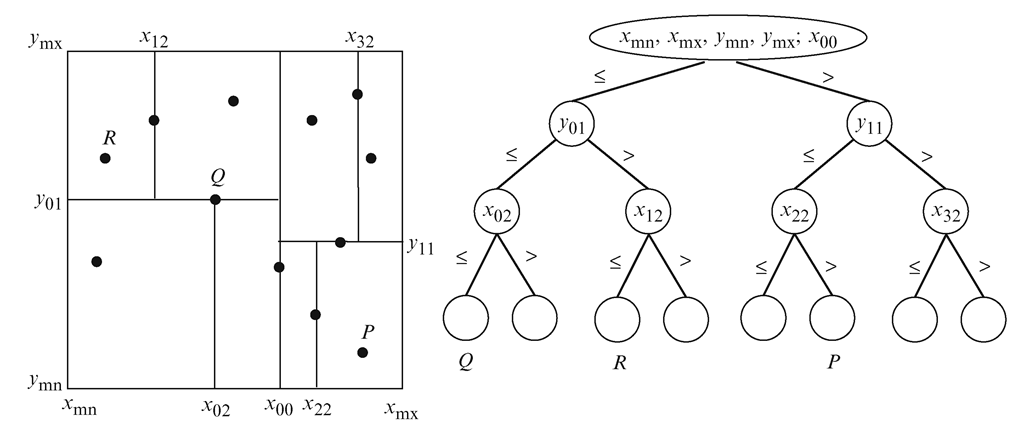
\includegraphics[width=\linewidth]{Figures/AABB}
	\caption{Esempio di albero di tipo AABB.}
	\label{AABB}
\end{figure}
%
\subsubsection{Struttura di tipo "\textit{Arbitrarily Oriented Bounding Box}"}
Il \ac{MBB} orientato arbitrariamente (\ac{AOBB}) è il rettangolo di delimitazione minimo, calcolato senza vincoli di orientazione.
%
\subsubsection{Struttura di tipo "\textit{Object Oriented Bounding Box}"}
Nel caso in cui un oggetto abbia un proprio sistema di coordinate locale, può essere utile memorizzare un rettangolo di selezione relativo a questi assi, che non richiede alcuna trasformazione quando cambia l'orientazione dell'oggetto stesso.

\subsection{Intersezione tra alberi di tipo AABB}
Per il rilevamento delle collisioni tra oggetti in due dimensioni, l'intersezione tra alberi di tipo \ac{AABB} è l'algoritmo più veloce per determinare se le due entità di gioco si sovrappongono o meno, e in che parti. Nello specifico, vengono controllate le posizioni delle \textit{i}-esime \ac{BB} nello spazio delle coordinate bidimensionali per vedere se si sovrappongono.

Il vincolo di allineamento dei rettangoli agli assi è presente per motivi di prestazioni, infatti, l'area di sovrapposizione tra due rettangoli non ruotati può essere controllata solo tramite confronti logici. I riquadri ruotati richiedono invece ulteriori operazioni trigonometriche, che sono più lente da calcolare. Inoltre, se si hanno entità che possono ruotare, le dimensioni dei rettangoli e/o sotto-rettangoli dovranno modificarsi in modo da avvolgere ancora l'oggetto, altrimenti si dovrà optare per un altro tipo di geometria di delimitazione, come le sfere (che sono invarianti alla rotazione).

% DA RISCRIVERE : CI SONO STATE MODIFICHE
Nel caso specifico, l'ombra dello pneumatico sarà rappresentata da un albero di tipo \ac{AABB} con una sola foglia. Ovvero si andrà a rappresentare lo pneumatico con una \ac{BB} avente lati uguali e rappresentanti il massimo ingombro che può avere nello spazio. Si andrà inoltre ad incrementare del 10\% ognuno di questi lati in modo da tenere conto dell'angolo di camber, che potrebbe portare i punti di campionamento del terreno fuori dall'ombra. La strada, contrariamente allo pneumatico, verrà tenuta come riferimento assoluto. In altre parole, una volta effettuata l'analisi sintattico-grammaticale del \textit{file} \ac{RDF}, verrà calcolato l'albero di tipo \ac{AABB}. Lo pneumatico si muoverà all'interno della \textit{mesh} e la sua ombra verrà ricalcolata e intersecata con l'albero \ac{AABB} per ottenere tutti i triangoli in corrispondenza della stessa.

Volendo intersecare due semplici \ac{BB}, quali 
\begin{equation*}
\begin{split}
A = \left[ \texttt{A.minX}, \texttt{A.maxX},  \texttt{A.minY}, \texttt{A.maxY} \right]\\
B = \left[ \texttt{B.minX}, \texttt{B.maxX},  \texttt{B.minY}, \texttt{B.maxY} \right]
\end{split}
\end{equation*}
verrà usata la seguente funzione:
\vspace{.8em}
\begin{pseudoc}
	function intersect(A,B) {
		return (A.minX <= B.maxX && A.maxX >= B.minX) &&
					 (A.minY <= B.maxY && A.maxY >= B.minY)
	}
\end{pseudoc}
\vspace{.5em}
\noindent
Volendo intersecare un albero di tipo \ac{AABB} e una semplice \ac{BB}, basterà ripetere a più step la funzione precedente lungo i rami dell'albero. Una volta arrivati a una o più foglia avremo tutti gli oggetti (o triangoli nel caso specifico) che sono posti in corrispondenza della \ac{BB} (od ombra dello pneumatico nel caso specifico). Questi triangoli verranno poi usati per determinare il piano strada locale e il punto di contatto virtuale dello pneumatico.

È importante notare che il metodo appena visto, presenta numerosi vantaggi:
\begin{itemize}
	\item Riduzione del numero di comparazioni da effettuare per ottenere l'intersezione \ac{BB}-albero \ac{AABB}. Il metodo presentato consente di ridurre logaritmicamente il numero di comparazioni necessarie per ottenere il risultato, dato che la \textit{mesh} può contenere decine di migliaia di triangoli.
	\item Riduzione del numero di triangoli da processare per ottenere il piano strada locale e il punto di contatto virtuale dello pneumatico. Infatti, vengono solamente processati quelli posti in corrispondenza dell'ombra dello pneumatico.
\end{itemize}
%
\section{Algoritmi geometrici}
%
La geometria computazionale è la branca dell'informatica che studia le strutture dati e gli algoritmi efficienti per la soluzione di problemi di natura geometrica e la loro implementazione al calcolatore. Storicamente, è considerato uno dei campi più antichi del calcolo, anche se la geometria computazionale moderna è uno sviluppo recente. I progressi compiuti nei campi computer grafica, del \ac{CAD}, del \ac{CAM} e nella visualizzazione matematica sono la ragione principale per lo sviluppo della geometria computazionale. Ad oggi, le sue applicazioni si trovano nella robotica, nella progettazione di circuiti integrati, nella visione artificiale, nel \ac{CAE} e nel \ac{GIS}. I rami principali della geometria computazionale sono:
\begin{itemize}
	\item \textit{Calcolo combinatorio} (o \textit{geometria algoritmica}), che si occupa di oggetti geometrici come entità discrete. Ad esempio, può essere utilizzato per determinare il poliedro o il poligono più piccolo che contiene tutti i punti forniti, o più formalmente, dato un insieme di punti, si deve determinare il più piccolo insieme convesso che li contenga tutti (problema dell'inviluppo convesso).
	\item \textit{Geometria di calcolo} numerica (o \ac{CAGD}), che si occupa principalmente di rappresentare oggetti del mondo reale in forme adatte per i calcoli informatici nei sistemi \ac{CAD} e \ac{CAM}. Questo ramo può essere considerato uno sviluppo della geometria descrittiva ed è spesso ritenuto un ramo della computer grafica o del \ac{CAD}. Entità importanti di questo ramo sono superfici e curve parametriche, come ad esempio le \textit{spline} e \textit{curve di Bézier}.
\end{itemize}
In questo capitolo saranno trattati tutti gli algoritmi che verranno utilizzati in seguito durante l'analisi geometrica dell'intersezione tra pneumatico e superficie stradale. Questi algoritmi sono la soluzione di alcuni semplici ma molto importanti problemi, che devono essere risolti in modo efficiente. In particolare, le intersezioni tra:
\begin{itemize}
	\item punto e segmento (nel piano);
	\item punto e cerchio (nel piano);
	\item segmento e circonferenza (nel piano);
	\item piano e piano (nello spazio);
	\item piano e segmento (nello spazio);
	\item piano e raggio (nello spazio);
	\item piano e triangolo (nello spazio);
	\item raggio e triangolo (nello spazio).
\end{itemize}
Essi saranno esaminati al fine di trovare la massima prestazione in termini di efficienza computazionale.
%
\subsection{Intersezione tra entità geometriche}
%
\subsubsection{Intersezione punto-segmento}
\label{punto-segmento}
Dato un punto $P = (x_p, y_p)$ e un segmento definito da due punti $A = (x_A, y_B)$ e $B = (x_B, y_B)$.

\begin{figure}[h!]
	\centering
	\begin{tikzpicture}
	\def\r{2};
	\coordinate (P) at (0.3,0.7);
	\coordinate (A) at (-2.0,0.0);
	\coordinate (B) at (+2.0,0.0);
	\draw[fill] (A) circle [radius=1pt] node[above] {$A$};
	\draw[fill] (B) circle [radius=1pt] node[above] {$B$};
	\draw[fill] (P) circle [radius=1pt] node[above] {$P$};
	\draw[thick](A) -- (B);
	\end{tikzpicture}
	\caption{Schema del problema di intersezione punto-segmento}
\end{figure}
\noindent
Per determinare se il punto $P$ è interno al segmento si eseguiranno i seguenti step:
\begin{enumerate}
	\item creazione di un vettore $\vv{AB}$ e di un vettore $\vv{AP}$;
	\item calcolo del prodotto vettoriale  $\vv{P_1P_2} \times  \vv{PP_1}$, se il modulo del vettore risultante è nullo allora il punto $P$ appartiene al segmento considerato;
	\item calcolo del prodotto scalare tra $\vv{AB}$ e $\vv{AP}$, se è nullo allora $P \equiv A$, se è pari al modulo di $\vv{AB}$ allora il $P \equiv B$, se è compreso tra 0 il modulo di $\vv{AB}$, allora il punto $P$ giace all'interno del segmento considerato.
\end{enumerate}
Lo pseudocodice che esegue questo tipo di test è riportato in \figurename{ \ref{pointsegment}}

\begin{figure}[h!]
	\hfill
	\begin{subfigure}{.45\textwidth}
		\centering
		\begin{tikzpicture}
		\coordinate (P0) at (0.3,0.7);
		\coordinate (P3) at (-0.7,0);
		\coordinate (A) at (-2.0,0.0);
		\coordinate (B) at (+2.0,0.0);
		\draw[fill] (P0) circle [radius=1pt] node[above] {\texttt{0}};
		\draw[fill] (A) circle [radius=1pt] node[above] {\texttt{1}};
		\draw[fill] (B) circle [radius=1pt] node[above] {\texttt{2}};
		\draw[fill] (P3) circle [radius=1pt] node[above] {\texttt{3}};
		\draw[thick](A) -- (B);
		\end{tikzpicture}
		\caption{\textit{Output} di tipo \texttt{integer}}
	\end{subfigure}
	\hfill
	\begin{subfigure}{.45\textwidth}
		\centering
		\begin{tikzpicture}
		\coordinate (P0) at (0.3,0.7);
		\coordinate (P3) at (-0.7,0);
		\coordinate (A) at (-2.0,0.0);
		\coordinate (B) at (+2.0,0.0);
		\draw[fill] (P0) circle [radius=1pt] node[above] {\texttt{false}};
		\draw[fill] (A) circle [radius=1pt] node[above] {\texttt{true}};
		\draw[fill] (B) circle [radius=1pt] node[above] {\texttt{true}};
		\draw[fill] (P3) circle [radius=1pt] node[above] {\texttt{true}};
		\draw[thick](A) -- (B);
		\end{tikzpicture}
		\caption{\textit{Output} di tipo \texttt{bool}}
	\end{subfigure}
	\hfill
	\caption{Schemi per l'\textit{output} dell'intersezione punto-segmento.}
\end{figure}
\begin{figure}[h!]
	\hfill
	\begin{subfigure}[t]{.45\linewidth}
	\raggedright
	\textit{Output} di tipo \texttt{integer}\\
	\vspace{.5em}
	\begin{pseudoc}
	if ( AB.cross(AP) > epsilon )
		{ return 0; }
	KAP = AB.dot(AP);
	if ( KAP < -epsilon )
		{ return 0; }
	if ( abs(KAP) < epsilon  )
		{ return 1; }
	KAB = AB.dot(AB);
	if ( KAP > KAB )
		{ return 0; }
	if ( abs(KAP-KAB) < epsilon )
		{ return 2; }
	return 3;
	\end{pseudoc}
	\end{subfigure}
	\hfill
	\begin{subfigure}[t]{.45\textwidth}
	\raggedright
	\textit{Output} di tipo \texttt{bool}\\
	\vspace{.5em}
	\begin{pseudoc}
	if ( AB.cross(AP) > epsilon )
		{ return false; }
	KAP = AB.dot(AP);
	if ( KAP < -epsilon )
		{ return false; };
	if ( abs(KAP) < epsilon )
		{ return true; }
	KAB = AB.dot(AB);
	if ( KAP > KAB ) 
		{ return false; }
	if ( abs(KAP-KAB) < epsilon )
		{ return true; }
	return true;
	\end{pseudoc}
	\end{subfigure}
	\hfill
	\caption{Schema del codice per l'intersezione punto-segmento.}
	\label{pointsegment}
\end{figure}
%
\subsubsection{Intersezione punto-cerchio}
Data una circonferenza con centro $C = (x_c, y_c)$ e raggio $r$, il problema consiste nel trovare se un generico punto $P = (x_p, y_p)$ è all'interno, all'esterno o corrispondente alla circonferenza.

\begin{figure}[h]
	\centering
	\begin{tikzpicture}
	\def\r{2};
	\coordinate (C) at (0,0) node[above left] {$C$};
	\draw[thick, fill=gray!10](C) circle (\r);
	\coordinate (P) at (-0.5,-1.5);
	\draw[fill] (C) circle [radius=1pt];
	\draw[fill] (P) circle [radius=1pt];
	\draw(C) -- (P)  node[above left] {$P$} node[pos=0.5, right] {$d$};
	\draw(C) -- ({sqrt(\r)},{sqrt(\r)}) node[pos=0.4, above] {$r$};
	\end{tikzpicture}
	\caption{Schema del problema di intersezione punto-cerchio.}
\end{figure}
La soluzione al problema è semplice: la distanza tra il centro della circonferenza $C$ e il punto $P$ è data dal teorema di Pitagora, ovvero:
\begin{equation}
	d=\sqrt{(x_p-x_c)^2 + (y_p-y_c)^2}
\end{equation}
Il punto $P$ è dunque interno alla circonferenza se $d<r$, appartiene alla circonferenza se $d=r$ ed esterno alla circonferenza se $d>r$. In maniera analoga ma più efficace da punto di vista computazionale si può confrontare $d^2$ con $r^2$. Il punto $P$ è dunque interno alla circonferenza se $d^2<r^2$,  appartiene alla circonferenza se $d^2=r^2$ ed esterno alla circonferenza se $d^2>r^2$. Pertanto, il confronto finale sarà tra il numero $(x_p-x_c)^2+(y_p-y_c)^2 $ e $r^2$.

Gli \textit{inputs} dell'algoritmo per l'intersezione punto-cerchio sono:
\begin{itemize}
	\item il centro della circonferenza $C = (x_c, y_c)$;
	\item il raggio della circonferenza $r$;
	\item il punto generico da analizzare $P=(x_p, y_p)$.
\end{itemize}
L'\textit{output} può essere un intero il cui valore risulta:
\begin{itemize}
	\item \texttt{0} se il punto è esterno alla circonferenza;
	\item \texttt{1} se il punto è interno alla circonferenza;
	\item \texttt{2} se il punto appartiene alla circonferenza.
\end{itemize}
Il valore in \textit{output} può essere anche una variabile booleana il cui valore è:
\begin{itemize}
	\item \texttt{false} se il punto è esterno alla circonferenza;
	\item \texttt{true} se il punto è interno o appartiene alla circonferenza.
\end{itemize}
%
\begin{figure}[h]
\hfill
	\begin{subfigure}{.45\textwidth}
	\centering
	\begin{tikzpicture}
	\def\r{2};
	\coordinate (C) at (0,0);
	\draw[thick, fill=gray!10](C) circle (\r);
	\draw[fill] (0,-0.5) circle [radius=1pt] node[above left] {\texttt{1}};
	\draw[fill] (-\r,0) circle [radius=1pt] node[above left] {\texttt{2}};
	\draw[fill] (3,0) circle [radius=1pt] node[above left] {\texttt{0}};
	\end{tikzpicture}
	\caption{\textit{Output} di tipo \texttt{integer}}
\end{subfigure}
\hfill
\begin{subfigure}{.45\textwidth}
	\centering
	\begin{tikzpicture}
	\def\r{2};
	\coordinate (C) at (0,0);
	\draw[thick, fill=gray!10](C) circle (\r);
	\draw[fill] (0,-0.5) circle [radius=1pt] node[above left] {\texttt{true}};
	\draw[fill] (-\r,0) circle [radius=1pt] node[above left] {\texttt{true}};
	\draw[fill] (3,0) circle [radius=1pt] node[above] {\texttt{false}};
	\end{tikzpicture}
	\caption{\textit{Output} di tipo \texttt{bool}}
\end{subfigure}
\hfill
\caption{Schemi per l'\textit{output} dell'intersezione punto-cerchio.}
\end{figure}
\begin{figure}[h]
\hfill
	\begin{subfigure}[t]{.475\linewidth}
	\raggedright
	\textit{Output} di tipo \texttt{integer}\\
	\vspace{.5em}
	\begin{pseudoc}
	d = (x_p-x_c)^2 + (y_p-y_c)^2;
	if ( d > r^2 ){ return  0; }
	else if ( d < r^2 ){ return 1; }
	else { return 2; }
	\end{pseudoc}
	\end{subfigure}
\hfill
	\begin{subfigure}[t]{.475\textwidth}
	\raggedright
	\textit{Output} di tipo \texttt{bool}\\
	\vspace{1em}
	\begin{pseudoc}
	d = (x_p-x_c)^2 + (y_p-y_c)^2;
	if ( d > r^2 ){ return  true; }
	else { return false; }
	\end{pseudoc}	
	\end{subfigure}
\hfill
\caption{Schemi del codice per l'intersezione punto-cerchio.}
\label{Pointcircle}
\end{figure}
%
\subsubsection{Intersezione segmento-circonferenza}
Per l'intersezione di un segmento, avente punto iniziale e finale rispettivamente in $P_0$ e $P_1$, con una circonferenza, avente centro $C=(x_c,y_c)$ e raggio $r$, è necessario prima di tutto riscrivere le equazioni di entrambe le entità. Il segmento viene momentaneamente riscritto come una retta del tipo:
\begin{equation}
ax+by=c
\label{eqretta}
\end{equation}
mentre la circonferenza come:
\begin{equation}
(x-x_c)^2 + (y-y_c)^2 = r^2
\end{equation}
Assumendo che il centro $C$ sia posto sull'origine, la precedente equazione si può semplificare come:
\begin{equation}
x^2 + y^2 = r^2
\label{eqcircle}
\end{equation}
\begin{figure}[h]
	\centering
	\begin{tikzpicture}
	\def\r{2};
	\coordinate (C) at (0,0);
	\coordinate (P0) at (-4,-1);
	\coordinate (P1) at (4,-1);
	\draw[thick, fill=gray!10](C) circle (\r);
	\draw[fill] (C) circle [radius=1pt];
	\draw[fill] (P0) circle [radius=1pt];
	\draw[fill] (P1) circle [radius=1pt];
	\draw[thick](P0) -- (P1) node[above] {$P_1$} node[pos=0, above] {$P_0$};
	\draw(C) -- ({sqrt(\r)},{sqrt(\r)}) node[pos=0.4, above] {$r$};
	\draw[fill] ({-sqrt(3)/2*\r},{-0.5*\r}) circle [radius=1pt] node[below left] {$(x_1,y_1)$};
	\draw[fill] ({sqrt(3)/2*\r},{-0.5*\r}) circle [radius=1pt] node[below right] {$(x_2,y_2)$};
	\end{tikzpicture}
	\caption{Schema del problema di intersezione punto-circonferenza.}
\end{figure}

Per trovare i termini $a$, $b$ e $c$ è necessario calcolare la direzione del segmento come differenza tra il punto finale e iniziale del segmento:
\begin{equation}
\vec{d} = P_1 - P_0 
\end{equation}
È neccessario anche trovare il vettore tra l'origine e il punto $P_1$:
\begin{equation}
\vec{P}_{O1} = P_1 - O
\end{equation}
I termini $a$, $b$ e $c$ saranno quindi pari a:
\begin{equation}
\begin{aligned}
	\begin{split}
		a =& \vec{d} \cdot \vec{d} \\
		b =& 2 (\vec{d} \cdot \vec{P}_{O1}) \\
		c =& \vec{P}_{O1} \cdot \vec{P}_{O1} - r^2
	\end{split}
\end{aligned}
\end{equation}
Risolvere l'equazione \ref{eqretta} per $x$ o $y$ è ora molto semplice. Basta infatti sostituirla nell'equazione \ref{eqcircle} per ottenere le soluzioni $(x_1, y_1)$ e $(x_2, y_2)$ con:
\begin{equation}
x_{1/2} = \frac{ac \pm b \sqrt{r^2 (a^2 + b^2)-c^2}}{a ^ 2 + b ^ 2}
\end{equation}
oppure:
\begin{equation}
y_{1/2} = \frac{bc \mp a \sqrt{r^2 (a^2 + b^2)-c^2}}{a ^ 2 + b ^ 2}
\end{equation}
Se $r^2 (a^2 + b^2)-c^2 \geq 0$ vale come una disuguaglianza stretta, esistono due punti di intersezione. Se invece vale $r^2 (a^2 + b^2)-c^2 = 0$, allora esiste solo un punto di intersezione e la linea è tangente alla circonferenza. Se la disuguaglianza debole non regge, la linea non interseca la circonferenza.

Dal punto di vista del codice, l'\textit{output} può essere un intero il cui valore può risultare:
\begin{itemize}
	\item \texttt{0} se la linea non interseca la circonferenza;
	\item \texttt{1} se la linea interseca la circonferenza in un solo punto, ovvero è tangente;
	\item \texttt{2} se la linea interseca la circonferenza in due punti.
\end{itemize}

Una volta ottenute il numero di intersezioni e le soluzioni $(x_1, y_1)$ e $(x_2, y_2)$ bisognerà controllare che queste siano all'interno del segnemto individuato inizialemnte dai punti $P_0$ e $P_1$. Per questo motivo si utilizzerà l'algoritmo di intersezione punto-segmento visto precedentemente in \ref{punto-segmento}.

\begin{figure}[h]
	\hfill
	\begin{subfigure}{.3\textwidth}
		\centering
		\begin{tikzpicture}
		\def\r{1.5};
		\coordinate (C) at (0,0);
		\coordinate (P0) at (-2,-1.75);
		\coordinate (P1) at (2,-1.75);
		\draw[thick, fill=gray!10](C) circle (\r);
		\draw(C) node {\texttt{0}};
		\draw[fill] (P0) circle [radius=1pt];
		\draw[fill] (P1) circle [radius=1pt];
		\draw[thick](P0) -- (P1) node[above] {$P_1$} node[pos=0, above] {$P_0$};
		\end{tikzpicture}
	\end{subfigure}
	\hfill
	\begin{subfigure}{.3\textwidth}
		\centering
		\begin{tikzpicture}
		\def\r{1.5};
		\coordinate (C) at (0,0);
		\coordinate (P0) at (-2,-1.5);
		\coordinate (P1) at (2,-1.5);
		\draw[thick, fill=gray!10](C) circle (\r);
		\draw(C) node {\texttt{1}};
		\draw[fill] (P0) circle [radius=1pt];
		\draw[fill] (P1) circle [radius=1pt];
		\draw[thick](P0) -- (P1) node[above] {$P_1$} node[pos=0, above] {$P_0$};
		\draw[fill] (0,-\r) circle [radius=1pt];
		\end{tikzpicture}
	\end{subfigure}
	\hfill
	\begin{subfigure}{.3\textwidth}
		\centering
		\begin{tikzpicture}
		\def\r{1.5};
		\coordinate (C) at (0,0);
		\coordinate (P0) at (-2,-0.75);
		\coordinate (P1) at (2,-0.75);
		\draw[thick, fill=gray!10](C) circle (\r);
		\draw(C) node {\texttt{2}};
		\draw[fill] (P0) circle [radius=1pt];
		\draw[fill] (P1) circle [radius=1pt];
		\draw[thick](P0) -- (P1) node[above] {$P_1$} node[pos=0, above] {$P_0$};
		\draw[fill] ({-sqrt(3)/2*\r},{-0.5*\r}) circle [radius=1pt];
		\draw[fill] ({sqrt(3)/2*\r},{-0.5*\r}) circle [radius=1pt];
		\end{tikzpicture}
	\end{subfigure}
	\hfill
	\caption{Schemi per l'\textit{output} dell'intersezione segmento-cerchio.}
\end{figure}
\begin{figure}[htbp]
	\centering
	\begin{subfigure}{.65\linewidth}
	\begin{pseudoc}
	a = d $\cdot$ d;
	b = 2 * (d $\cdot$ P_O1);
	c = P_O1 $\cdot$ P_O1 - r^2;
	discriminant = r^2 * (a^2 + b^2) - c^2;
	if ( a <= epsilon || discriminant < 0.0 ) {
		IntPt_1 = (quiteNaN, quiteNaN);
		IntPt_2 = (quiteNaN, quiteNaN);
		return 0;
	} else if ( abs(discriminant) < epsilon ) {
		t = - b / (2 * a);
		IntPt_1 = P_1 + t * d;
		IntPt_2 = (quiteNaN, quiteNaN);
		return 1;
	} else {
		t = (-b + sqrt(discriminant)) / (2 * a);
		IntPt_1 = P_1 + t * d;
		t = (-b - sqrt(discriminant)) / (2 * a);
		IntPt_2 = P_1 + t * d;
		return 2;
	}
	\end{pseudoc}
	\end{subfigure}
	\caption{Schema dello pseudocodice per l'intersezione segmento-cerchio.}
\end{figure}
%
\subsubsection{Intersezione piano-piano}
Nello spazio delle coordinate tridimensionali, due piani $P_1$ e $P_2$ o sono paralleli o si intersecano creando una singola retta $L$. Sia $P_i$ con $i = 1,2$ descritto da un punto $V_i$ e un vettore normale $\vec{n}_i$. L'equazione implicita del piano sarà dunque:
\begin{equation}
\vec{n}_i \cdot P + d_i = 0
\end{equation}
dove $P = (x, y, z)$. I piani $P_1$ e $P_2$ sono paralleli ogni volta che i loro normali vettori $\vec{n}_1$ e $\vec{n}_2$ sono paralleli. Questo equivale alla condizione che $\vec{n}_1 \times \vec{n}_2 = 0$. Quando i piani non sono paralleli, $\vec{u} = \vec{n}_1 \times \vec{n}_2$ è il vettore di direzione della linea di intersezione $L$. Si noti che $\vec{u}$ è perpendicolare sia a $\vec{n}_1$ che a $\vec{n}_2$, e quindi è parallelo a entrambi i piani.

\begin{figure}
	\centering
	\tdplotsetmaincoords{70}{110}
	\begin{tikzpicture}[tdplot_main_coords,font=\sffamily]
	\draw[-latex] (0,0,0) -- (4,0,0) node[left] {$x$};
	\draw[-latex] (0,0,0) -- (0,4,0) node[below] {$y$};
	\draw[-latex] (0,0,0) -- (0,0,4) node[left] {$z$};
	\tdplotsetrotatedcoords{45}{0}{0}
	\begin{scope}[tdplot_rotated_coords]
	\draw[fill=gray!10,opacity=0.6] (-3,0,-3) -- (-3,0,3) -- (3,0,3) -- (3,0,-3) -- cycle;
	\end{scope}
	\tdplotsetrotatedcoords{90}{45}{0}
	\begin{scope}[tdplot_rotated_coords]
	\draw[fill=gray!10,opacity=0.5] (-3,-3,0) -- (-3,3,0) -- (3,3,0) -- (3,-3,0) -- cycle;
	\draw[thick](-3,{3/sqrt(2)},0) coordinate(x) --(3,{-3/sqrt(2)},0);
	\end{scope}
	\node[anchor=south east,align=center] (line) at (3,-1.5,3.5) {$L$};
	\draw[-latex] (line) to[out=0,in=135] (x);
	\end{tikzpicture}
	\caption{Schemi del problema di intersezione piano-piano.}
\end{figure}

Dopo aver calcolato $\vec{n}_1 \times \vec{n}_2$, per determinare univocamente la linea di intersezione, è necessario trovare un punto di essa. Cioè, un punto $P_0 = (x_0, y_0, z_0)$ che si trova in entrambi i piani. Si può trovare una soluzione comune delle equazioni implicite per $P_1$ e $P_2$. Ci sono solo due equazioni nelle tre incognite poiché il punto $P_0$ può trovarsi ovunque sulla linea monodimensionale $L$. Quindi è necessario aggiungere un altro vincolo da risolvere per un $P_0$ specifico. Esistono diversi modi per farlo, il più semplice è attraverso l'aggiunta di un terzo piano $P_3$ avente equazione implicita $\vec{n}_3 \cdot P = 0$ dove $\vec{n}_3 = \vec{n}_1 \times \vec{n}_2$ e $d_3 = 0$ (ovvero passa attraverso l'origine). Questo metodo è funzionante poiché: 
\begin{itemize}
	\item $L$ è perpendicolare a $P_3$ e quindi lo interseca;
	\item i vettori $\vec{n}_1$, $\vec{n}_2$ e $\vec{n}_3$ sono linearmente indipendenti.
\end{itemize}
Pertanto, i piani $P_1$, $P_2$ e $P_3$ si intersecano in un unico punto $P_0$ che deve trovarsi su $L$. 

\begin{figure}
	\centering
	\tdplotsetmaincoords{70}{110}
	\begin{tikzpicture}[tdplot_main_coords]
	\draw[-latex] (0,0,0) -- (4,0,0) node[left] {$x$};
	\draw[-latex] (0,0,0) -- (0,4,0) node[below] {$y$};
	\draw[-latex] (0,0,0) -- (0,0,4) node[left] {$z$};
	\draw[fill=gray!10,opacity=0.6] (-3,0,-3) -- (-3,0,3) -- (3,0,3) -- (3,0,-3) -- cycle;
	\draw[fill=gray!10,opacity=0.5] (-3,-3,0) -- (-3,3,0) -- (3,3,0) -- (3,-3,0) -- cycle;
	\draw[dashed] (-3,0,0)--(3,0,0);
	\draw[-stealth,thick] (0,0,0) -- (2,0,0);
	\draw[-stealth,thick] (0,0,0) -- (0,2,0) node[above] {$\vec{n}_1$};
	\draw[-stealth,thick] (0,0,0) -- (0,0,2) node[left] {$\vec{n}_2$};
	\draw(2,.1,0) node[right] {$\vec{n}_3$};
	\end{tikzpicture}
	\caption{Vettori dei piani $P_1$, $P_2$ e della retta $L$.}
\end{figure}

Nello specifico, la formula per l'intersezione di tre piani è:
\begin{equation}
P_0 =  \frac{-d_1(\vec{n}_2 \times \vec{n}_3) - d_2(\vec{n}_3 \times \vec{n}_1) - d_3(\vec{n}_1 \times \vec{n}_2)}{\vec{n}_1 \cdot (\vec{n}_2 \times \vec{n}_3)}
\end{equation}
e ponendo $d_3 = 0$ per $P_3$, si ottiene:
\begin{equation}
P_0 =  \frac{-d_1(\vec{n}_2 \times \vec{n}_3) - d_2(\vec{n}_3 \times \vec{n}_1)}{\vec{n}_1 \cdot (\vec{n}_2 \times \vec{n}_3)}
=
\frac{(d_2\vec{n}_1 - d_1\vec{n}_2) \times \vec{n}_3}{(\vec{n}_1 \times \vec{n}_2) \cdot \vec{n}_3}
=
\frac{(d_2\vec{n}_1 - d_1\vec{n}_2) \times \vec{u}}{|\vec{u}|^2}
\end{equation}
pertanto l'equazione parametrica per la retta $L$ sarà:
\begin{equation}
L(s) =
\frac{(d_2\vec{n}_1 - d_1\vec{n}_2) \times \vec{u}}{|\vec{u}|^2}+s\vec{u}
\end{equation}
dove $\vec{u}=\vec{n}_1 \times \vec{n}_2$.

\begin{figure}[htbp]
	\centering
	\begin{subfigure}{.65\linewidth}
		\begin{pseudoc}
	u = n_1 $\times$ n_2;
	if ( u.norm() > epsilon ) {
		d_1 = - V_1 $\cdot$ n_1;
		d_2 = - V_2 $\cdot$ n_2;
		u_1 = d_1 * n_1;
		u_2 = - d_2 * n_2;
		P_0 = (u1 + u2) $\times$ u / (u $\cdot$ u);
		return true;
	} else {
		return false;
	}
		\end{pseudoc}
	\end{subfigure}
	\caption{Schema dello pseudocodice per l'intersezione piano-piano.}
\end{figure}
%
\subsubsection{Piano-Segmento e Piano-Raggio}
Nello spazio delle coordinate tridimensionali, una linea $L$ può essere o parallela a un piano $P$ o può intersecarlo in un singolo punto. Sia $L$ data dall'equazione parametrica:
\begin{equation}
P(t) = P_0 + t(P_1-P_0) = P_0 + t\vec{u}
\end{equation}
mentre il piano $P$ sia dato da un punto $V_0$ appartenente ad esso e da un vettore normale $\vec{n} = (a,b,c)$. Per prima cosa è necessario controllare se $L$ è parallelo a $P$ verificando se $\vec{n}\cdot\vec{u} = 0$, il che significa che il vettore di direzione della linea $\vec{u}$ è perpendicolare al piano normale $\vec{n}$. Se questo è vero, allora $L$ e $P$ sono paralleli e non si intersecano, oppure $L$ giace totalmente nel piano $P$. Disgiunzione o coincidenza possono essere determinate testando se in $P$ esiste un punto specifico di $L$, per esempio $P_0$, ovvero se soddisfa l'equazione di linea implicita:
\begin{equation}
\vec{n} \cdot (P_0-V_0) = 0
\end{equation}
Se la linea e il piano non sono paralleli, allora $L$ e $P$ si intersecano in un unico punto $P(t_I)$. Nel punto di intersezione, il vettore $P(t)-V_0 = \vec{w} + t\vec{u}$ è perpendicolare a $\vec{n}$, dove $\vec{w} = P_0-V_0$. Ciò equivale alla condizione del prodotto scalare:
\begin{equation}
\vec{n} \cdot (\vec{w}+t\vec{u}) = 0
\end{equation}
Risolvendo si ottiene:
\begin{equation}
t_I = -\frac{\vec{n}\cdot\vec{w}}{\vec{n}\cdot\vec{u}}
=
-\frac{\vec{n}\cdot(V_0-P_0)}{\vec{n}\cdot(P_1-P_0)}
\end{equation}
Se la linea $L$ è un segmento finito da $P_0$ a $P_1$, è sufficiente verificare che $0 \leq t_I \leq 1$ per dimostrare che vi sia un'intersezione tra il segmento e il piano. Per raggio, c'è invece un'intersezione con il piano quando $t_I \geq 0$.

\begin{figure}[htbp]
	\centering
	\tdplotsetmaincoords{70}{110}
	\begin{tikzpicture}[tdplot_main_coords]
	\draw[-latex] (0,0,0) -- (4,0,0) node[left] {$x$};
	\draw[-latex] (0,0,0) -- (0,4,0) node[below] {$y$};
	\draw[-latex] (0,0,0) -- (0,0,4) node[left] {$z$};
	
	\draw[fill=gray!10,opacity=0.5] (-3,-3,0) -- (-3,3,0) -- (3,3,0) -- (3,-3,0) -- cycle;
	\draw[-stealth,thick] (0,-0.75,3.25) node[above] {$P_0$} -- (0,1.25,1.25) node[above right] {$P_1$};
	\draw (0,-0.5,2.25) node[below left] {$\vec{w}$};
	\draw (0,0.25,2.25) node[above right] {$\vec{u}$};
	\draw[-stealth,thick] (0,0,0) -- (0,-0.75,3.25);
	\draw[dashed] (0,1.25,1.25) -- (0,2.5,0);
	\draw[fill] (0,2.5,0) circle [radius=1pt];
	\draw (0,2.5,0) node[below left] {$P(t_I)$};
	\draw (0,2,0.5) node[right] {$P(t)$};
	\draw[fill] (0,2,.5) circle [radius=1pt];
	\draw[-stealth,thick] (1,-2,0) -- (1,-2,2) node[left] {$\vec{n}$};
	\end{tikzpicture}
	\caption{Vettori dei piani $P_1$, $P_2$ e della retta $L$.}
\end{figure}
\begin{figure}[htbp]
	\centering
	\begin{subfigure}{.5\linewidth}
		\begin{pseudoc}
	u = P_1 - P_0;
	t = n $\cdot$ (V_0 - P_0) / (u $\cdot$ n);
	if ( t >= 0 && t <= 1 ) {
		P_tI = P_0 + u * t;
		return true;
	} else {
		return false;
	}
		\end{pseudoc}
	\end{subfigure}
	\caption{Schema dello pseudocodice per l'intersezione piano-segmento.}
\end{figure}
%
\subsubsection{Intersezione piano-triangolo}
Per risolvere l'intersezione piano triangolo basta usare la soluzione precedentemente trovata per il problema dell'intersezione tra piano e segmento. Nello specifico, basta trattare i lati del triangolo come tre segmenti distinti e per ognuno di esso applicare la funzione per l'intersezione piano-segmento. Vi saranno tre possibili soluzioni:
\begin{itemize}
	\item il triangolo non viene intersecato dal piano;
	\item il triangolo viene intersecato dal piano in uno dei suoi tre vertici;
	\item il triangolo viene intersecato dal piano, formando quindi due punti d'intersezione nel suo perimetro.
\end{itemize}

\begin{figure}[htbp]
	\centering
	\begin{subfigure}{.73\linewidth}
		\begin{pseudoc}
	if ( intersectSegmentPlane( n, V_0, 1, IntPt_1 ))
	{ IntPts.push_back(IntPt1); }
	if ( intersectSegmentPlane( n, V_0, 2, IntPt2 ))
	{ IntPts.push_back(IntPt2); }
	if ( intersectSegmentPlane( n, V_0, 3, IntPt3 ))
	{ IntPts.push_back(IntPt3); }
	if ( IntPts.size() == 2 ) 
	{ return true; }
	else if ( IntPts.size() == 0 ) 
	{ return false; }
	else 
	{ return false; }
		\end{pseudoc}
	\end{subfigure}
	\caption{Schema dello pseudocodice per l'intersezione piano-triangolo.}
\end{figure}
%
\subsubsection{Intersezione raggio-triangolo}
Dato un triangolo avente vertici $(A,B,C)$ e un raggio $R$ con origine $R_O$ e direzione $\vec{R}_D$, il problema consiste nel capire se il raggio colpisce o meno il triangolo e, in tal caso, trovare il punto di intersezione $P$.
%
\begin{figure}[htbp]
	\centering
	\begin{tikzpicture}
	\coordinate [label=left:$A$] (A) at (-1,-0.5);
	\coordinate [label=above:$B$] (B) at (1,1);
	\coordinate [label=right:$C$] (C) at (2.2,-1);
	\draw[fill=gray!10] (A) -- (B) -- (C) -- (A);
	\def\xp{0.4};
	\def\yp{-0.2};
	\def\xd{-1};
	\def\yd{1};
	\def\mag{1.7};
	\coordinate [label=above right:$P$] (P) at (\xp,\yp);
	\coordinate [label={[shift={(0.1,0.1)}]$\vec{R}_D$}] (RD) at (\xp+\xd,\yp+\yd);
	\coordinate [label=above:$R_O$] (RO) at (\xp+\xd*\mag,\yp+\yd*\mag);
	\draw[fill] (P) circle [radius=1pt];
	\draw[fill] (RO) circle [radius=1pt];
	\draw[-stealth] (RO) -- (RD);
	\draw[dashed] (RD) -- (P);
	\end{tikzpicture}
	\caption{Schema del problema di intersezione raggio-triangolo.}
\end{figure}
%
Negli ultimi decenni, sono stati proposti numerosi algoritmi per risolvere questo problema, esistono quindi diverse soluzioni al problema di intersezione raggio-triangolo. Tre degli algoritmi più importanti sono:
\begin{itemize}
	\item l'algoritmo di \textit{Badouel};
	\item l'algoritmo di \textit{Segura};
	\item l'algoritmo di \textit{M\"oller} e \textit{Trumbore}.
\end{itemize}
\noindent
Come \citeauthor{RayTriangle} afferma in \cite{RayTriangle}, l'algoritmo di M\"oller-Trumbore è il più veloce quando il piano normale e/o il piano di proiezione non sono stati precedentemente memorizzati, come nel caso specifico di questa tesi.

La teoria alla base di questo algoritmo è spiegata estensivamente in \cite{Moller}. In particolare, l'algoritmo sfrutta la parametrizzazione di $P$, il punto di intersezione, in termini delle coordinate baricentriche, ovvero:
\begin{equation}
	P = wA + uB + vC
\end{equation}
Dato che $w = 1-u-v$, si può quindi scrivere:
\begin{equation}
	P = (1-u-v)A + uB + vC
\end{equation}
e sviluppando si ottiene:
\begin{equation}
	P = A-uA-vA+uB+vC = A+u(B-A)+v(C-A)
	\label{eq1}
\end{equation}
Si noti che $(B-A)$ e $(C-A)$ sono i bordi $AB$ e $AC$ del triangolo $ABC$. L'intersezione $P$ può anche essere scritta usando l'equazione parametrica del raggio:
\begin{equation}
	P = R_O + t\vec{R}_D
	\label{eq2}
\end{equation}
dove $t$ è la distanza dall'origine del raggio all'intersezione $P$. Sostituendo $P$ nell'equazione \ref{eq1} con l'equazione del raggio si ottiene:
\begin{equation}
	\begin{split}
	\begin{aligned}
		R_O + t\vec{R}_D =& A+u(B-A)+v(C-A)\\
		O - A =& -tD+u(B-A)+v(C-A)
	\end{aligned}
	\end{split}
	\label{eq3}
\end{equation}
Sul membro a sinistra si hanno le tre incognite $(t,u,v)$ moltiplicate per tre termini noti $(B-A, C-A, D)$. Si può riorganizzare questi termini e presentare l'equazione \ref{eq3} usando la seguente notazione:
\begin{equation}
	\begin{bmatrix}
	-D & (B-A) & (C-A)
	\end{bmatrix}
	\begin{bmatrix}
	t \\
	u \\
	v
	\end{bmatrix} = R_O - A
	\label{eq4}
\end{equation}
Si immagini ora di avere un punto $P$ all'interno del triangolo. Se si trasforma il triangolo in qualche modo (ad esempio traslandolo, ruotandolo o scalandolo), le coordinate del punto $P$ espresse nel sistema di coordinate cartesiane tridimensionali $(x,y,z)$ cambieranno. D'altra parte, se si esprime la posizione di $P$ usando le coordinate baricentriche, le trasformazioni applicate al triangolo non influenzeranno le coordinate baricentriche del punto di intersezione. Se il triangolo viene ruotato, ridimensionato, allungato o traslato, le coordinate $(u,v)$ che definiscono la posizione di $P$ rispetto ai vertici $(A,B,C)$ non cambieranno. L'algoritmo di M\"oller-Trumbore sfrutta proprio questa proprietà. Infatti, gli autori hanno definito un nuovo sistema di coordinate in cui le coordinate di $P$ non sono definite in termini di $(x,y,z)$ ma in termini di $(u,v)$. La somma tra le coordinate baricentriche non può essere maggiore di 1 ($u + v \leq 1$), infatti esprimono le coordinate dei punti definiti all'interno di un triangolo unitario, ovvero un triangolo definito nello spazio $(u,v)$ dai vertici $(0,0)$, $(1,0)$, $(0,1)$.

\begin{figure}[htbp]
	\centering
	\hfill
	\begin{subfigure}[t]{.45\linewidth}
		\begin{tikzpicture}
		\coordinate (O) at (0,0,0);
		\def\axisl{3}
		\draw[-stealth] (O) -- (\axisl,0,0) node[below]{$x$};
		\draw[-stealth] (O) -- ({sqrt(\axisl)},{sqrt(\axisl)},0) node[above]{$y$};
		\draw[-stealth] (O) -- (0,\axisl,0) node[left]{$z$};
		\coordinate [label=below:$C$] (V1) at ({\axisl/1.5},0.5,0);
		\coordinate [label=above:$B$] (V2) at ({sqrt(\axisl)/1.5},{3.3/1.8},0);
		\coordinate [label={[shift={(-0.15,0)}]$A$}] (V3) at (0.3,0.6,0);
		\draw[fill=gray!10] (V1) -- (V2) -- (V3) -- (V1);
		
		\def\xp{1};
		\def\yp{1};
		\def\xd{-1};
		\def\yd{0.8};
		\def\mag{1.7};
		\coordinate [label=above:$P$] (P) at (\xp,\yp);
		\coordinate [label={[shift={(-0.3,-0.5)}]$\vec{R}_D$}] (RD) at (\xp+\xd*1.1,\yp+\yd*1.1);
		\coordinate [label=above:$R_O$] (RO) at (\xp+\xd*\mag*1.1,\yp+\yd*\mag*1.1);
		\draw[fill] (P) circle [radius=1pt];
		\draw[fill] (RO) circle [radius=1pt];
		\draw[-stealth] (RO) -- (RD);
		\draw[dashed] (RD) -- (P);
		\end{tikzpicture}
	\end{subfigure}
	\hfill
	\begin{subfigure}[t]{.45\linewidth}
		\begin{tikzpicture}
		\coordinate (O) at (0,0,0);
		\def\axisl{3}
		\draw[-stealth] (O) -- (\axisl,0,0) node[below]{$\alpha$};
		\draw[-stealth] (O) -- ({sqrt(\axisl)},{sqrt(\axisl)},0) node[above]{$\beta$};
		\draw[-stealth] (O) -- (0,\axisl,0) node[left]{$\gamma$};
		\coordinate [label={[below,font=\tiny]:$1$}] (V1) at ({\axisl/1.5},0,0);
		\coordinate [label={[shift={(-0.1,0.0)},font=\tiny]:$1$}] (V2) at ({sqrt(\axisl)/1.5},{sqrt(\axisl)/1.5},0);
		\coordinate (V3) at (0,0,0);
		\draw[fill=gray!10] (V1) -- (V2) -- (V3) -- (V1);
				
		\def\xp{0.7};
		\def\yp{0.35};
		\def\xd{0};
		\def\yd{1};
		\def\mag{1.7};
		\coordinate [label=right:$P$] (P) at (\xp,\yp);
		\coordinate [label={[shift={(-0.35,-0.15)}]$\vec{R}_D$}] (RD) at (\xp+\xd,\yp+\yd);
		\coordinate [label=above:$R_O$] (RO) at (\xp+\xd*\mag,\yp+\yd*\mag);
		\draw[fill] (P) circle [radius=1pt];
		\draw[fill] (RO) circle [radius=1pt];
		\draw[-stealth] (RO) -- (RD);
		\draw[dashed] (RD) -- (P);
		\end{tikzpicture}
	\end{subfigure}
	\hfill
	\caption{Cambiamento di coordinate nell'algoritmo di M\"oller-Trumbore.}
\end{figure}

Geometricamente, si è appena chiarito il significato di $u$ e $v$. Si consideri ora l'elemento $t$. Esso è il terzo asse del sistema di coordinate $u$ e $v$ appena introdotto. Si sa inoltre che $t$ esprime la distanza dall'origine del raggio a $P$, il punto di intersezione. Si è quindi creato un sistema di coordinate che consentirà di esprimere univocamente la posizione del punto d'intersezione $P$ in termini di coordinate baricentriche e distanza dall'origine del raggio a quel punto sul triangolo.

M\"oller e Trumbore spiegano che la prima parte dell'equazione \ref{eq4} (il termine $O-A$) può essere vista come una trasformazione che sposta il triangolo dalla sua posizione spaziale mondiale originale all'origine (il primo vertice del triangolo coincide con l'origine). L'altro lato dell'equazione ha l'effetto di trasformare il punto di intersezione dallo spazio $(x,y,z)$ nello spazio $(t,u,v)$ come spiegato precedentemente.

Per risolvere l'equazione \ref{eq4}, M\"oller e Trumbore hanno usato una tecnica conosciuta in matematica come regola di Cramer. La regola di Cramer fornisce la soluzione a un sistema di equazioni lineari mediante il determinante. La regola afferma che se la moltiplicazione di una matrice $M$ per un vettore colonna $X$ è uguale a un vettore colonna $C$, allora è possibile trovare $X_i$ (l'$i$-esimo elemento del vettore colonna $X$) dividendo il determinante di $M_i$ per il determinante di $M$. Dove $M_i$ è la matrice formata sostituendo la sua colonna di $M$ con il vettore colonna $C$. Usando questa regola si ottiene;
\begin{equation}
\begin{bmatrix}
t \\
u \\
v
\end{bmatrix} = 
\frac{1}{\begin{vmatrix}-D & E_1 & E_2\end{vmatrix}}
\begin{bmatrix}
\begin{vmatrix}T & E_1 & E_2\end{vmatrix} \\
\begin{vmatrix}-D & T & E_2\end{vmatrix} \\
\begin{vmatrix}-D & E_1 & T\end{vmatrix}
\end{bmatrix}
\label{eq5}
\end{equation}
dove $T=O-A$, $E_1=B-A$ ed $E_2=C-A$. Il prossimo passo è trovare un valore per questi quattro determinanti. Il determinante (di una matrice $3 \times 3$) non è altro che un triplo prodotto scalare, quindi si può riscrivere l'equazione precedente come:
\begin{equation}
\begin{bmatrix}
t \\
u \\
v
\end{bmatrix} 
= \frac{1}{(D \times E_2) \cdot E_1}
\begin{bmatrix}
(T \times E_1) \cdot E_2 \\
(D \times E_2) \cdot T \\
(T \times E_1) \cdot D
\end{bmatrix}
= \frac{1}{P \cdot E_1}
\begin{bmatrix}
Q \cdot E_2 \\
P \cdot T \\
Q \cdot D
\end{bmatrix}
\end{equation}
dove $P = (D \times E_2)$ e $Q = (T \times E_1)$. Come si può vedere ora è facile trovare i valori $t$, $u$ e $v$.

\begin{figure}
	\hfill
	\begin{subfigure}{.3\linewidth}
		\centering
		\begin{tikzpicture}
		\coordinate (A) at (-1,-0.5);
		\coordinate (B) at (1,1);
		\coordinate (C) at (2.2,-1);
		\draw[fill=gray!10] (A) -- (B) -- (C) -- (A);
		\def\xp{0};
		\def\yp{-0.2};
		\def\xd{0};
		\def\yd{1};
		\def\mag{1.7};
		\coordinate [label=right:\texttt{true}] (P) at (\xp,\yp);
		\coordinate (RD) at (\xp+\xd,\yp+\yd);
		\coordinate (RO) at (\xp+\xd*\mag,\yp+\yd*\mag);
		\draw[fill] (P) circle [radius=1pt];
		\draw[fill] (RO) circle [radius=1pt];
		\draw[-stealth] (RO) -- (RD);
		\draw[dashed] (RD) -- (P);
		\end{tikzpicture}
	\end{subfigure}
	\hfill
	\begin{subfigure}{.3\linewidth}
		\centering
		\begin{tikzpicture}
		\coordinate (A) at (-1,-0.5);
		\coordinate (B) at (1,1);
		\coordinate (C) at (2.2,-1);
		\draw[fill=gray!10] (A) -- (B) -- (C) -- (A);
		\def\xp{0};
		\def\yp{0.25};
		\def\xd{0};
		\def\yd{1};
		\def\mag{1.7};
		\coordinate [label=below right:\texttt{true}] (P) at (\xp,\yp);
		\coordinate (RD) at (\xp+\xd,\yp+\yd);
		\coordinate (RO) at (\xp+\xd*\mag,\yp+\yd*\mag);
		\draw[fill] (P) circle [radius=1pt];
		\draw[fill] (RO) circle [radius=1pt];
		\draw[-stealth] (RO) -- (RD);
		\draw[dashed] (RD) -- (P);
	\end{tikzpicture}
	\end{subfigure}
	\hfill
	\begin{subfigure}{.3\linewidth}
	\centering
	\begin{tikzpicture}
		\coordinate (A) at (-1,-0.5);
		\coordinate (B) at (1,1);
		\coordinate (C) at (2.2,-1);
		\draw[fill=gray!10] (A) -- (B) -- (C) -- (A);
		\def\xp{-0.3};
		\def\yp{0.25};
		\def\xd{0};
		\def\yd{1};
		\def\mag{1.7};
		\coordinate [label=left:\texttt{false}] (P) at (\xp,\yp);
		\coordinate (RD) at (\xp+\xd,\yp+\yd);
		\coordinate (RO) at (\xp+\xd*\mag,\yp+\yd*\mag);
		\draw[fill] (P) circle [radius=1pt];
		\draw[fill] (RO) circle [radius=1pt];
		\draw[-stealth] (RO) -- (RD);
		\draw[dashed] (RD) -- (P);
	\end{tikzpicture}
	\end{subfigure}
	\hfill
	\caption{Schemi per l'\textit{output} dell'intersezione punto-cerchio.}
\end{figure}
\begin{figure}[htbp]
	\centering
	\begin{subfigure}{.65\linewidth}
	\begin{pseudoc}
	E_1 = B - A;
	E_2 = C - A;
	A = R_D $\times$ E_2;
	D = A $\cdot$ E_1;
	if ( D > epsilon ) {
		T = R_0 - A;
		u = A $\cdot$ T;
		if ( u < 0.0 || u > D ) return false;
		B = T $\times$ E_1;
		v = B $\cdot$ R_D;
		if (v < 0.0 || u + v > D) return false;
	} else if ( D < -epsilon ) {
		T = R_0 - A;
		u = A $\cdot$ T;
		if (u > 0.0 || u < D) return false;
		B = T $\times$ E_1;
		v = B $\cdot$ R_D;
		if ( v > 0.0 || u + v < D ) return false;
	} else {
		return false;
	}
	t = ( B $\cdot$ E_2 ) / D;
	if ( t > 0.0 ) {
		P = Q + D * t;
		return true;
	} else {
		return false;
	}
	\end{pseudoc}
	\end{subfigure}
	\caption{Schema dello pseudocodice per l'intersezione raggio-triangolo con \textit{back-face culling}.}
\end{figure}